% Options for packages loaded elsewhere
\PassOptionsToPackage{unicode}{hyperref}
\PassOptionsToPackage{hyphens}{url}
\PassOptionsToPackage{dvipsnames,svgnames,x11names}{xcolor}
\documentclass[
  11pt,
  a4paper,
]{article}
\usepackage{xcolor}
\usepackage[margin=1in]{geometry}
\usepackage{amsmath,amssymb}
\setcounter{secnumdepth}{5}
\usepackage{iftex}
\ifPDFTeX
  \usepackage[T1]{fontenc}
  \usepackage[utf8]{inputenc}
  \usepackage{textcomp} % provide euro and other symbols
\else % if luatex or xetex
  \usepackage{unicode-math} % this also loads fontspec
  \defaultfontfeatures{Scale=MatchLowercase}
  \defaultfontfeatures[\rmfamily]{Ligatures=TeX,Scale=1}
\fi
\usepackage{lmodern}
\ifPDFTeX\else
  % xetex/luatex font selection
\fi
% Use upquote if available, for straight quotes in verbatim environments
\IfFileExists{upquote.sty}{\usepackage{upquote}}{}
\IfFileExists{microtype.sty}{% use microtype if available
  \usepackage[]{microtype}
  \UseMicrotypeSet[protrusion]{basicmath} % disable protrusion for tt fonts
}{}
\makeatletter
\@ifundefined{KOMAClassName}{% if non-KOMA class
  \IfFileExists{parskip.sty}{%
    \usepackage{parskip}
  }{% else
    \setlength{\parindent}{0pt}
    \setlength{\parskip}{6pt plus 2pt minus 1pt}}
}{% if KOMA class
  \KOMAoptions{parskip=half}}
\makeatother
\usepackage{longtable,booktabs,array}
\newcounter{none} % for unnumbered tables
\usepackage{calc} % for calculating minipage widths
% Correct order of tables after \paragraph or \subparagraph
\usepackage{etoolbox}
\makeatletter
\patchcmd\longtable{\par}{\if@noskipsec\mbox{}\fi\par}{}{}
\makeatother
% Allow footnotes in longtable head/foot
\IfFileExists{footnotehyper.sty}{\usepackage{footnotehyper}}{\usepackage{footnote}}
\makesavenoteenv{longtable}
\usepackage{graphicx}
\makeatletter
\newsavebox\pandoc@box
\newcommand*\pandocbounded[1]{% scales image to fit in text height/width
  \sbox\pandoc@box{#1}%
  \Gscale@div\@tempa{\textheight}{\dimexpr\ht\pandoc@box+\dp\pandoc@box\relax}%
  \Gscale@div\@tempb{\linewidth}{\wd\pandoc@box}%
  \ifdim\@tempb\p@<\@tempa\p@\let\@tempa\@tempb\fi% select the smaller of both
  \ifdim\@tempa\p@<\p@\scalebox{\@tempa}{\usebox\pandoc@box}%
  \else\usebox{\pandoc@box}%
  \fi%
}
% Set default figure placement to htbp
\def\fps@figure{htbp}
\makeatother
\setlength{\emergencystretch}{3em} % prevent overfull lines
\providecommand{\tightlist}{%
  \setlength{\itemsep}{0pt}\setlength{\parskip}{0pt}}
\usepackage[]{natbib}
\bibliographystyle{plainnat}
\usepackage{bookmark}
\IfFileExists{xurl.sty}{\usepackage{xurl}}{} % add URL line breaks if available
\urlstyle{same}
\hypersetup{
  pdftitle={From Self-Stabilizing Dynamics to Conscious Experience},
  pdfauthor={Jorge Simão},
  colorlinks=true,
  linkcolor={blue},
  filecolor={Maroon},
  citecolor={blue},
  urlcolor={blue},
  pdfcreator={LaTeX via pandoc}}

\title{From Self-Stabilizing Dynamics to Conscious Experience}
\usepackage{etoolbox}
\makeatletter
\providecommand{\subtitle}[1]{% add subtitle to \maketitle
  \apptocmd{\@title}{\par {\large #1 \par}}{}{}
}
\makeatother
\subtitle{A Physical and Ontological Framework for Embodied
Consciousness}
\author{Jorge Simão}
\date{Version 0.2 --- August 2026}

\begin{document}
\maketitle
\begin{center}\small\textbf{Status:} Conceptual foundation paper, version 0.2. Mechanistic, empirical, and ontological claims are distinguished throughout.\end{center}

\begin{abstract}
This paper proposes a research programme linking embodied cognition,
dynamical neuroscience, and a restricted identity hypothesis about
consciousness. Its mechanistic proposal is that an embodied cognitive
system continually stabilizes viable perception--action relations under
perturbations arising from the environment, body, action, and its own
activity. Repeated stabilization across spatial and temporal scales
produces hierarchically organized invariants and a dynamically
maintained internal physical world. The framework treats
activation-correlation structures (ACS)---time-evolving, multiscale
relations among neural or physical populations---as a candidate
mesoscopic bridge among microscopic events, population dynamics,
behavior, phenomenological transitions, and measurable electromagnetic
manifestations. Coherent electromagnetic organization is therefore
treated as a macroscopic manifestation of coordinated electrical
dynamics, not as an independently sufficient consciousness-producing
field. Its empirical hypothesis is that multidimensional ACS profiles
will add reproducible explanatory and predictive value for perceptual
stability and consciousness level beyond activity, power, anatomy, and
conventional connectivity alone. Its ontological proposal is that a
qualifying self-stabilizing physical organization does not generate a
second entity called experience: its intrinsic existence is hypothesized
to be the subjective aspect. This identity proposal relocates rather
than deductively solves the hard problem and leaves a substantial
qualification problem. Seven operationalized predictions, seven
experimental programmes, comparisons with neighbouring theories, and
twelve objections specify how the framework could be developed or
disconfirmed without treating evidence for its mechanism as proof of its
ontology.
\end{abstract}

\section{Introduction}\label{introduction}

Consciousness research faces a coordination problem as much as an
explanatory one. Neuroscience can relate reports and behavioural
responsiveness to recurrent processing, widespread access, neural
complexity, and changing patterns of integration. Embodied and enactive
approaches explain perception and cognition through
organism--environment coupling. Dynamical systems theory describes
transient coordination and metastability. Philosophy asks why any of
these public processes should have a subjective aspect. These lines of
work constrain one another, yet they are often presented as competing
complete explanations or as enquiries that can proceed independently.

This paper develops a narrower synthesis. An embodied cognitive system
must continually maintain workable relations among its sensory states,
actions, internal activity, bodily needs, and environment. Maintenance
here is not passive constancy. It is a temporally extended process of
correction, exploration, compensation, and reorganization under
perturbation. Patterns that remain useful across repeated
transformations become increasingly invariant. Their organization is not
exhausted by the activity of individual units; it also depends on
relations among units and on how those relations persist and change
across timescales. The paper calls these evolving relational patterns
\textbf{activation-correlation structures (ACS)}.

In nervous systems, ACS are implemented by physical neural activity.
Ionic currents necessarily have electromagnetic (EM) consequences, and
measurements such as local field potentials, EEG, and MEG sample
projections of coordinated electrical dynamics \citep{nunez2006}. The
present framework does not extract the field from its generators and
assign it an independent power to produce consciousness. It treats
coherent EM organization as the most directly measurable macroscopic
manifestation of coordinated electrical dynamics, while leaving open
whether field-level variables have causal roles not captured by current
neural measurements.

The most speculative step is ontological. The framework hypothesizes
that the intrinsic existence of a qualifying, self-stabilizing physical
organization is its subjective aspect. A nervous system does not build a
miniature picture for a further observer. It maintains an
organism-centred physical world of relations. On the identity proposal,
the subject and the experienced world are aspects of the ongoing
existence of that organized process. This move belongs near identity
theory and Russellian-monist families rather than constituting a novel
metaphysical proof \citep{smart1959, strawson2006, chalmers2013}. Its
possible contribution is a restricted mechanistic route to the kind of
organization that might qualify.

The resulting chain is:

\begin{quote}
embodied coupling → perturbation and correction → dynamic homeostasis →
metastable stabilization → hierarchical invariants → multiscale ACS →
measurable EM organization → a restricted empirical correlate hypothesis
→ an ontological identity proposal.
\end{quote}

Every arrow before the last two is intended to become a mechanistic or
empirical research question. The final identity is a philosophical
hypothesis. Confirmation of an ACS marker would not, by itself,
establish the identity claim. Conversely, disagreement with the ontology
need not invalidate the mechanistic programme.

\begin{figure}
\centering
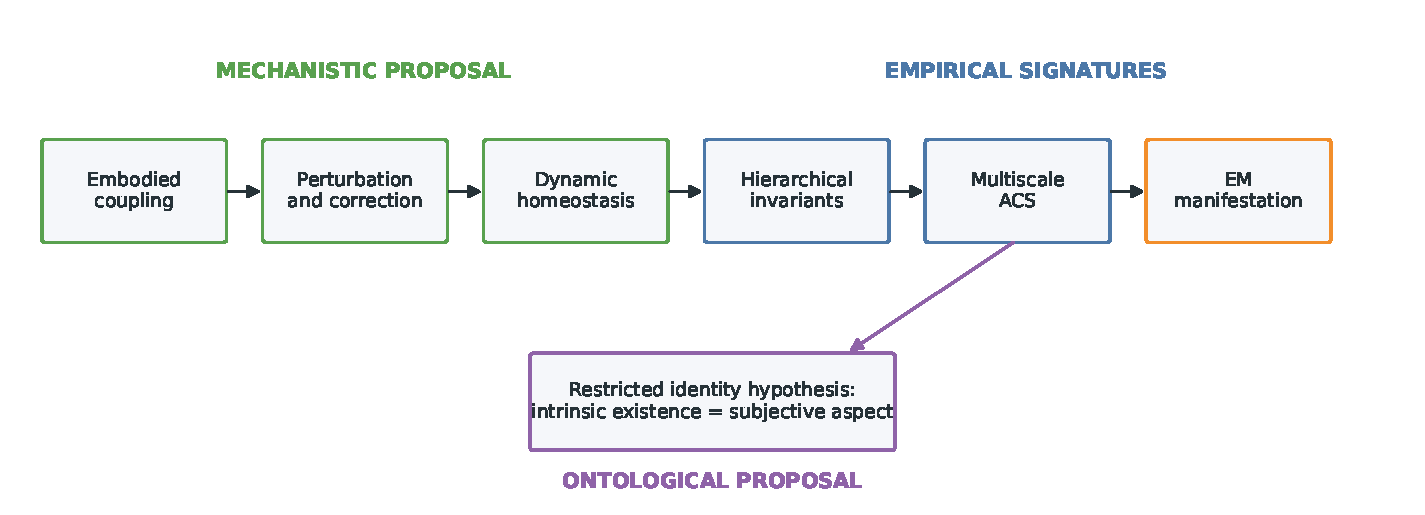
\includegraphics[width=0.95\linewidth,height=\textheight,keepaspectratio,alt={The proposed chain distinguishes embodied mechanism, empirical signatures, and ontology. Arrows indicate research dependencies rather than established entailments.}]{figures/figure1_mechanistic_chain.pdf}
\caption{The proposed chain distinguishes embodied mechanism, empirical
signatures, and ontology. Arrows indicate research dependencies rather
than established entailments.}
\end{figure}

\section{Scope, claims, and epistemic
levels}\label{scope-claims-and-epistemic-levels}

The framework makes three kinds of claim that must be evaluated
separately.

\begin{enumerate}
\def\labelenumi{\arabic{enumi}.}
\item
  \textbf{Mechanistic proposal.} Cognition can be modelled as active
  stabilization of viable organism--environment relations.
  Self-generated and external perturbations provide variation; dynamic
  homeostasis prevents silence, saturation, rigidity, and uncontrolled
  activity; repeated stabilization produces invariants. Prediction-error
  or free-energy minimization may implement parts of this process, but
  no unique objective function is assumed.
\item
  \textbf{Empirical hypothesis.} Some regularities associated with
  stable percepts and global conscious organization are better captured
  by multiscale relational trajectories than by isolated activity
  values. ACS measures should therefore add out-of-sample predictive
  value, show structured changes under perturbation, and generalize
  where specified in Section 12. This is testable even if ACS is
  eventually replaced by a better relational construct.
\item
  \textbf{Ontological proposal.} A qualifying self-stabilizing physical
  organization is identical with, rather than a cause of, subjective
  existence. This does not follow from the empirical hypotheses. It is
  constrained by them only insofar as a defensible identity requires a
  principled account of what organization is being identified.
\end{enumerate}

The paper is a conceptual foundation, not a report of new experimental
results. It does not present a unique mathematical definition of
consciousness, a consciousness score, or a classification of present
animals, organoids, or artificial systems. It uses \emph{internal
physical world} for a causally active, physically instantiated
organization of organism-relevant relations, and \emph{ontological
realization} for the proposal that the organization's intrinsic
existence is the subjective aspect. Neither term denotes a hidden
observer or an extra substance.

\section{Cognition as self-stabilizing embodied
dynamics}\label{cognition-as-self-stabilizing-embodied-dynamics}

\subsection{Perception as
stabilization}\label{perception-as-stabilization}

Passive-encoding metaphors begin with an input, transform it, and end
with a representation. Embodied systems do not begin or end at those
boundaries. Their movements alter the next sensory sample; posture,
attention, autonomic state, and prior activity alter what can be
sampled; and the environment responds on its own timescale. Perception
is therefore better approached as the maintenance of a determinate but
revisable organization within a closed causal process. Sensorimotor and
enactive theories make related claims: perceptual capacities depend on
structured relations between possible actions and sensory consequences,
and cognition is a form of situated sense-making
\citep{oregan2001, noe2004, varela1991, thompson2007}.

\emph{Stabilization} does not mean that activity becomes constant or
that the system discovers a final equilibrium. It means that selected
relations remain within a functional regime despite disturbances. A
perceived cup can remain the same usable object while retinal input
changes with saccades, lighting, occlusion, and grasping. The stable
item is not a pixel array but a structured set of relations that
supports discrimination and action. The account is compatible with
determinate perceptual organization without positing an internal
spectator: reciprocal constraints among current input, memory, recurrent
state, body, and expected consequences can settle into one of several
context-sensitive organizations.

Four sources of perturbation matter. \textbf{Environmental
perturbations} include motion, noise, occlusion, and other agents.
\textbf{Bodily perturbations} include changing posture, fatigue, pain,
arousal, and internal physiology. \textbf{Action-generated
perturbations} include the sensory consequences of looking, reaching,
speaking, or withdrawing. \textbf{Endogenous perturbations} include
spontaneous activity, memory intrusion, exploratory variability, and
changes in attention. A cognitive architecture that remained useful only
under one fixed input would not be stable in the relevant sense.

Stabilization relates perception, prediction, control, action, and
correction without making them synonyms. Perception is the current
organization of relevant relations. Prediction estimates how those
relations may evolve, especially where delays make purely reactive
control inadequate. Control selects interventions that keep variables or
relations within viable regimes. Action changes the coupled system.
Correction uses the resulting discrepancy or loss of viability to revise
activity and future action. Predictive processing and active inference
offer influential formalisms for parts of this loop
\citep{clark2013, friston2010}. The present framework treats error or
free-energy minimization as possible implementations of stabilization,
not as its sole definition.

\subsection{Action and sensorimotor
closure}\label{action-and-sensorimotor-closure}

Closed perception--action loops are developmentally and organizationally
central because they provide interventions. Through action, a system can
learn which sensory regularities covary with its own movements, which
remain independent, and which actions restore a viable relation. This
turns observation into causal sampling. A reaching error can be
corrected, an occluded object can be viewed from another angle, and an
aversive internal state can motivate withdrawal or regulation.

The claim is not that overt action is required at every moment of
experience. Dreaming, imagery, paralysis, and temporary sensory
disconnection make that stronger claim implausible. The more defensible
claim is that the architecture capable of maintaining such episodes was
formed and is ordinarily maintained through embodied coupling. Once
established, recurrent activity, memory, and predictive organization can
temporarily sustain an internal physical world without current overt
movement. Even during paralysis, internal bodily regulation and neural
activity continue; nevertheless, these facts should not be used to
define away counterexamples. The developmental claim must be tested
against cases of congenital motor limitation and unusual sensory
histories.

Closure is also graded. A thermostat has a closed loop, but its
variables, timescales, repertoire, and learned organization are
extremely limited. Sensorimotor closure is therefore neither sufficient
for cognition nor a shortcut to consciousness. Its proposed role is to
ground relations and permit action-dependent stabilization.

\subsection{Perturbation, self-perturbation, and
metastability}\label{perturbation-self-perturbation-and-metastability}

An adaptive system needs variation as well as stability. Too little
perturbation can produce rigidity or habituation; too little
stabilization can produce noise, chaotic wandering, or loss of
functional identity. This tension motivates a
\textbf{self-perturbation--stabilization} principle: endogenous
variation supplies candidate states and actions, while selection and
regulation preserve organizations that remain viable and informative.
Randomness alone is not exploration, and persistence alone is not
cognition. The relevant regime combines bounded novelty with
recoverability.

Metastability provides an appropriate dynamical vocabulary. A metastable
state has a finite dwell time: it is stable enough to coordinate a
perception, intention, or action, yet remains capable of transition.
Coordination dynamics uses metastability to describe coexistence between
tendencies toward integration and independent activity
\citep{kelso1995}. Neural models and recordings also motivate
transient-state descriptions rather than a succession of permanent
attractors \citep{rabinovich2008, deco2017}. The framework therefore
expects multiple compatible organizations, context-sensitive dwell
times, and continuous adjustment rather than convergence to a single
optimum.

Perturbation is not merely an experimental nuisance. It is a way to
identify the causal organization of a system. Two systems may show the
same unperturbed activity yet differ in how they deform, recover, or
reorganize. Recovery time, transition path, and preservation of
task-relevant relations can therefore be more informative than a static
snapshot. The experimental programme uses external perturbations,
lesions, reversible inhibition, and closed-loop intervention for this
reason.

\subsection{Dynamic homeostasis}\label{dynamic-homeostasis}

Static constancy would be a poor objective for a nervous system.
Permanent high activity would saturate response ranges and obscure
differences; permanent depression or silence would remove functional
differentiation. Perfectly fixed correlations could preserve structure
only by eliminating sensitivity to new information. \textbf{Dynamic
homeostasis} instead means maintaining neural, bodily, and relational
variables within functional regimes while preserving enough variability
to encode, explore, learn, and reorganize.

At a minimal level, suppose a regulated variable (z\_i(t)) has a viable
interval rather than a single set point:

\[
z_i(t) \in [z_i^{-},z_i^{+}]
\]

for most of an interval relevant to the system. Regulation may minimize
excursions outside the interval while also preserving response variance,
for example through a provisional objective

\[
J = -\sum_i w_i\,\ell\!\left(z_i;z_i^{-},z_i^{+}\right)
    + \lambda_V V(x)
    + \lambda_R R(x),
\]

where (ell) penalizes non-viable excursions, (V(x)) rewards informative
variation, and (R(x)) rewards recoverability after perturbation. This is
not offered as a neural law. It makes explicit why stabilization cannot
be reduced to minimizing variance or freezing activity.

Known biology supplies related but non-equivalent mechanisms.
Homeostatic synaptic plasticity can counter destabilizing changes in
neural activity across local and network scales \citep{turrigiano2012}.
Excitation--inhibition regulation, intrinsic excitability, synaptic
scaling, neuromodulation, and plasticity can contribute on different
timescales. Allostasis emphasizes anticipatory regulation rather than
reaction after deviation, while interoceptive systems link large-scale
brain organization to regulation of the body
\citep{kleckner2017, tschantz2022}. The framework draws on these
phenomena but does not claim that dynamic homeostasis is identical to
any one of them.

Local adaptation and global regulation must coexist. If every unit
independently fixes its mean activity, population-level organization may
be lost; if only a global variable is controlled, local populations may
saturate or fall silent. A useful architecture should preserve relative
differences and task-relevant structure while maintaining bounded
activity, adequate entropy, and the capacity for future change. This
creates experimentally separable failure modes: saturation, silence,
rigid low-entropy repetition, unstable high-entropy activity, or loss of
recoverability.

\subsection{Hierarchical abstraction through invariant
pickup}\label{hierarchical-abstraction-through-invariant-pickup}

The central learning proposal can be expressed as a sequence. First,
fast local patterns stabilize over short intervals. Second, regularities
that recur across noise, viewpoint, action, and context survive repeated
perturbations. Third, other processes become selectively sensitive to
what remains stable across those lower-level changes. Fourth, slower or
more encompassing dynamics maintain increasingly invariant relations.
Fifth, an abstraction becomes a history of successful stabilization
across a family of transformations.

This hierarchy can be formalized provisionally by layer- or
scale-indexed state (h\_t\^{}\{(ell)\}), characteristic time ( au\_ell),
and perturbation radius (r\_ell):

\[
h_{t+1}^{(\ell)} = F^{(\ell)}\!\left(h_t^{(\ell)},h_t^{(\ell-1)},h_t^{(\ell+1)},a_t,\xi_t\right),
\]

\[
\tau_1 < \tau_2 < \cdots < \tau_L,
\qquad
r_1 < r_2 < \cdots < r_L.
\]

The inequalities are hypotheses to test, not anatomical laws. A
hierarchy can arise through spatial scale, temporal scale, recurrent
depth, causal organization, or their combination. Higher invariance need
not reside in a physically deeper cortical layer, and slower is not
always more abstract.

Examples illustrate the intended progression. Edge-like regularities
survive small local changes; object organizations survive viewpoint and
partial occlusion; places survive changing paths and lighting;
affordances survive variations in the motor route that realizes them;
other agents remain identifiable across motion and expression; social
situations preserve roles across different participants; self-models
integrate interoception, action history, memory, and social feedback;
abstract concepts preserve relational structure across superficially
different instances. Representational similarity analysis provides one
family of methods for testing whether relational geometry is preserved
across such transformations \citep{nili2014}.

Prediction becomes necessary when stabilization occurs across delayed
loops. Sensory, neural, and motor delays mean that a correction based
only on the present sample can arrive too late. The companion
mechanistic theory therefore proposes that reliable prediction may
emerge as \textbf{delayed stabilization}: maintaining a future viable
relation requires anticipating the consequences of action and
environmental change. This does not deny predictive coding. It makes a
specific empirical ordering claim: robust prediction should depend on
representations already stable under task-irrelevant perturbations, and
directly optimized prediction is not the only route by which
anticipatory dynamics may develop.

\subsection{Internal physical worlds}\label{internal-physical-worlds}

The nervous system does not construct a small inner picture. It
maintains a physically instantiated organization of relations: among
sensory regularities, possible actions, body state, remembered events,
expected outcomes, values, and other agents. Calling this an
\textbf{internal physical world} emphasizes six properties.

First, it is physical: it is realized in ongoing neural, bodily, and
field dynamics, not in an abstract description floating free of
implementation. Second, it is causally active: its current organization
constrains attention, action, memory, and autonomic regulation. Third,
it is externally constrained: successful stabilization depends on
regularities that survive contact with an environment not created by the
organism. Fourth, it is partly autonomous: recurrence, memory, and
prediction permit imagery, planning, dreaming, and error. Fifth, it
spans timescales, from transient sensory organization to persistent self
and world models. Sixth, it is centred on the organism's body, possible
actions, and viability.

``World'' here denotes structured relational scope, not veridical
completeness. Illusions and hallucinations remain internal physical
organizations, but their relations are less directly constrained by
current external causes. A photograph or database also contains
world-related structure, but need not maintain it through
self-stabilizing causal dynamics. The construct therefore combines
content, dynamics, embodiment, and maintenance rather than treating
representational resemblance as sufficient.

The decisive anti-homuncular statement is:

\begin{quote}
The conscious subject is not an additional entity observing the internal
world. The proposal is that the subject and experienced world are
aspects of the ongoing existence of that organized physical process.
\end{quote}

This is the paper's identity hypothesis, not an empirical conclusion
smuggled into the mechanistic description. A reader may accept internal
physical worlds as a useful model of cognition while rejecting their
proposed identity with experience.

\section{Activation-correlation
structures}\label{activation-correlation-structures}

\subsection{Motivation and role}\label{motivation-and-role}

Neural state is often summarized by firing rates, amplitudes, spectral
power, or localized activation. These quantities are indispensable, but
many cognitive properties concern relations: which populations
coordinate, with what lag and direction, in which frequency ranges, for
how long, and how the arrangement reconfigures. Dynamic
functional-connectivity research illustrates both the promise and the
methodological hazards of treating time-varying relations as scientific
objects \citep{hutchison2013}. ACS generalizes that intuition across
measurement modalities and scales.

An ACS is a time-evolving, multiscale relational structure implemented
by physical activity. It may include pairwise and lagged correlations,
phase synchrony, directed dependencies, recurrence, higher-order
interactions, community structure, integration and segregation,
cross-frequency relations, persistence, and transition structure. It is
intended as a mesoscopic bridge: microscopic events implement population
activity; population relations form measurable structures; structures
constrain metastable cognitive states and behaviour; their electrical
implementation produces measurable EM manifestations.

ACS does not make neurons or absolute activity unimportant. A
correlation pattern cannot exist without variables that vary, and
identical normalized correlations may accompany very different energy,
excitability, or causal regimes. The empirical question is whether
relational organization adds explanatory value beyond those variables.

\subsection{Minimal multiscale
formalism}\label{minimal-multiscale-formalism}

Let the state of (n) measured neural or physical populations be

\[
x(t) \in \mathbb{R}^{n}.
\]

For observation window ( au) and relational measure (m), define

\[
C_{\tau}^{(m)}(t)
=
\mathcal{R}^{(m)}
\left(
x(t') : t' \in [t-\tau,t]
\right).
\]

(mathcal\{R\}\^{}\{(m)\}) may estimate correlation, lagged mutual
information, phase coupling, transfer entropy, recurrence, a directed
graphical relation, or a higher-order interaction. The multiscale ACS is
the indexed family

\[
\mathcal{A}(t)
=
\left\{
C_{\tau}^{(m)}(t)
\right\}_{\tau \in T,\,m \in M}.
\]

This definition separates the research construct (mathcal\{A\}) from any
estimator. A Pearson correlation matrix at one window width is an
initial operationalization, not the ACS itself. Different modalities
impose different sampling rates, spatial mixing, noise models, and
causal limitations. EEG phase relations, calcium-imaging recurrence,
spiking transfer entropy, and fMRI connectivity cannot be treated as
interchangeable observations of a single exact object.

\subsection{ACS space and metastable
trajectories}\label{acs-space-and-metastable-trajectories}

To say that cognition evolves in ACS space is a modelling claim: some
cognitive regularities may be captured more naturally by trajectories
through relational organization than by trajectories of isolated
activations. An ACS trajectory can visit regions associated with a
stable percept, action policy, bodily state, or disconnected dream
episode. Context may shift the absolute activity while preserving part
of the relational geometry.

A metastable episode can be described by relatively slow structural
deformation:

\[
D\!\left(\mathcal{A}(t+\Delta t),\mathcal{A}(t)\right) < \varepsilon
\]

for a finite dwell interval. (D) might compare weighted graphs,
representational dissimilarity matrices, simplicial structures,
recurrence plots, or learned embeddings. A transition involves a
transient increase in structural change, not necessarily a total loss of
organization. Dwell-time distributions, transition probabilities, and
recovery trajectories matter as much as average stability.

\begin{figure}
\centering
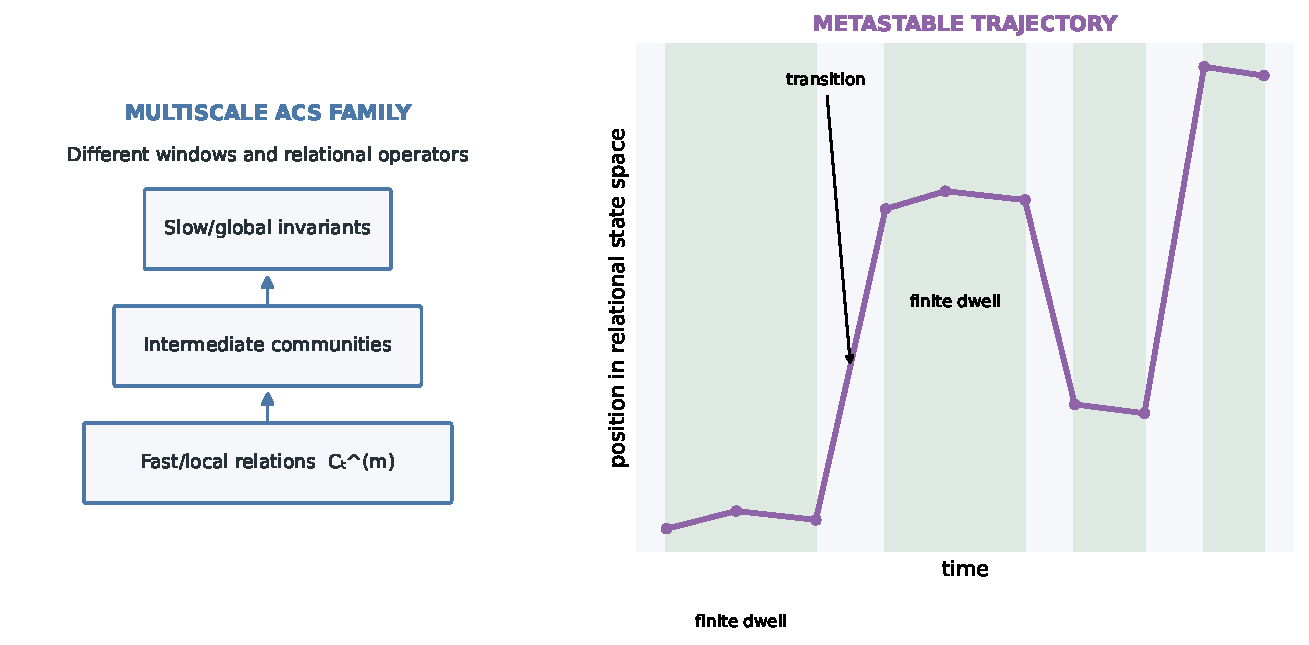
\includegraphics[width=0.92\linewidth,height=\textheight,keepaspectratio,alt={ACS is an indexed family of relational descriptions. Metastable episodes are finite regions of relatively slow deformation separated by transitions.}]{figures/figure2_acs_multiscale.pdf}
\caption{ACS is an indexed family of relational descriptions. Metastable
episodes are finite regions of relatively slow deformation separated by
transitions.}
\end{figure}

\subsection{Candidate dimensions and
limitations}\label{candidate-dimensions-and-limitations}

No consciousness score is proposed. Instead, an ACS profile may include
coherence, differentiation, integration, modularity, recurrence,
hierarchical depth, multiscale persistence, transition richness,
controllability, sensorimotor closure, robustness under perturbation,
and adaptability after perturbation. These dimensions can conflict: high
coherence may reduce differentiation; strong persistence may become
rigidity; rich transitions may become instability. The expected regime
is a structured profile, not maximization of every axis.

Several limitations follow. Relations depend on variable selection and
scale. Common drivers and volume conduction can create spurious
correlation. Sliding windows impose bias and temporal resolution.
Directed measures require assumptions that may not hold. Higher-order
estimators demand large samples. A learned ACS embedding may predict
well while remaining difficult to interpret. Analyses must therefore
include surrogate data, estimator sensitivity, preregistered windows
where possible, nested cross-validation, measurement-error models, and
baselines that contain raw activity, spectrum, anatomy, and conventional
connectivity. ACS earns a role only through reproducible incremental
value.

\section{Electromagnetic manifestation of organized
dynamics}\label{electromagnetic-manifestation-of-organized-dynamics}

Neural signalling involves ionic currents. Coordinated electrical
activity therefore has electromagnetic consequences, and EEG, MEG,
electrocorticography, and local field potentials provide different
projections of source organization \citep{nunez2006}. This physical
continuity motivates a modest claim:

\begin{quote}
Coherent electromagnetic organization is the most directly measurable
macroscopic manifestation of coordinated electrical dynamics, not
necessarily an independently causal or sufficient substrate of
consciousness.
\end{quote}

The claim differs from theories that identify a global EM field as the
integrative seat of consciousness or assign it a distinctive causal role
\citep{pockett2000, mcfadden2020}. Here, the relevant candidate is the
complete organized physical process: cellular currents, synaptic and
population dynamics, bodily and environmental coupling, and their field
manifestations. Abstracting the field from its generators may discard
causal organization just as abstracting a correlation matrix from its
signals can.

The difference is empirical where perturbation permits mediation
analysis. An external EM intervention will ordinarily change neural
activity; it is therefore incoherent to demand a manipulation that
changes the field while leaving the generating ACS literally unchanged.
The relevant questions are whether changes in conscious content or level
are statistically mediated by measurable changes in neural ACS, and
whether field-level variables explain reproducible residual effects
after sufficiently sensitive neural measurement. A residual would favour
an independent field-level causal contribution, although unmeasured
neural change would remain an alternative. Full mediation would support
the manifestation view but would not prove metaphysical identity.

\section{Consciousness as ontological
realization}\label{consciousness-as-ontological-realization}

The mechanistic sections describe how an internal physical world could
be maintained. The empirical sections ask which relational signatures
accompany perceptual stability and consciousness level. Neither answers
why there is something it is like for the system. The ontological
proposal begins by refusing a production metaphor: a qualifying physical
organization does not first exist non-experientially and then create a
second object called experience. Its intrinsic existence is hypothesized
to be the subjective aspect.

\emph{Intrinsic existence} means the organization as it exists and acts,
not merely as represented by an external model. \emph{Ontological
realization} means identity between that existence and subjectivity, not
causal generation across an unexplained gap. This resembles mind--brain
identity theory \citep{smart1959} and sits near Russellian-monist views
that distinguish structural descriptions of physics from the intrinsic
nature of what realizes them \citep{strawson2006, chalmers2013}. The
paper does not claim novelty for that move.

The proposed restriction is mechanistic. Not every correlation,
controller, oscillator, or field is assumed to qualify. Candidate
organization includes self-stabilizing causal closure across internal
and embodied variables, dynamic homeostasis, differentiation with
integration, multiscale recurrence, counterfactual robustness, and an
internally maintained world centred on the system's own viability. These
features are offered as a research profile, not necessary and sufficient
conditions.

This restriction avoids indiscriminate attribution but creates a
\textbf{qualification problem}: why should these organizations, and not
simpler or differently organized ones, have an intrinsic aspect? It also
leaves boundary and unity problems. If an ACS decomposes into modules,
why is there one subject rather than many? If two systems couple, when
do they form one organization? The framework cannot claim that the
combination problem is solved ``by construction''; it replaces a
universal combination problem with a restricted but still difficult
individuation problem.

\section{Qualia, language games, and the long
spectrum}\label{qualia-language-games-and-the-long-spectrum}

\subsection{Language-game thesis}\label{language-game-thesis}

Ordinary and scientific language uses contrasts such as
conscious/unconscious, experience/no experience, red/not red, pain/no
pain, and self/non-self. Such predicates coordinate reports, diagnosis,
action, and social expectations. Following the language-game insight
that a term's role depends on practices of use \citep{wittgenstein1953},
their practical sharpness need not reveal sharp natural boundaries.

Language can impose binary predicates on processes that are continuous,
multidimensional, hysteretic, or organized by family resemblance.
Clinical categories may be discrete because decisions must be made, even
when underlying physiology changes gradually. Colour names divide a
structured perceptual space for communication. ``Conscious'' may
sometimes mean reportable, responsive, awake, remembered, or morally
considerable. These uses should not be conflated.

Linguistic analysis does not establish phenomenal continuity. The
independent argument is mechanistic: candidate dimensions such as
differentiation, recurrence, sensorimotor closure, temporal persistence,
and self-modelling can vary separately and gradually. If experience is
identical with qualifying organization, then changes in organization
motivate---but do not logically guarantee---a graded and
multidimensional phenomenology.

\subsection{A multidimensional long
spectrum}\label{a-multidimensional-long-spectrum}

A single ladder from ``less'' to ``more'' consciousness is premature.
Philosophical and comparative work has argued for separating level from
content and for multidimensional animal-consciousness profiles
\citep{bayne2016, birch2020}. The present framework distinguishes at
least: presence or global level, richness of content, selfhood, temporal
continuity, reportability, cognitive access, valence, and moral
relevance. None is assumed to determine all the others.

The empirical domain forms a long spectrum: ordinary waking states;
attention and inattention; dreaming; sedation and anaesthesia; seizures
and disorders of consciousness; infants and developing organisms;
non-human animals and simple nervous systems; neural cultures and
organoids; future embodied artificial systems; and hypothetical minimal
physical organizations. Listing these cases is not an assertion that all
are conscious. It replaces an immediate yes/no verdict with questions
about what kind of internal physical world, if any, is maintained; on
which timescales; with what stability, differentiation, bodily
relevance, and capacity for perturbation recovery.

\begin{figure}
\centering
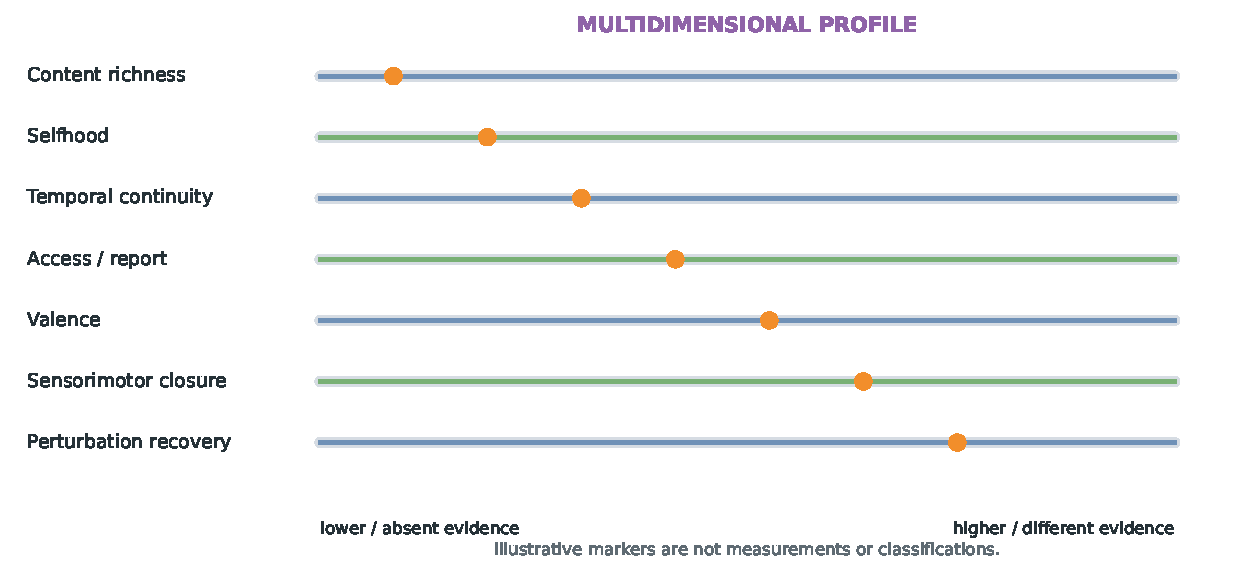
\includegraphics[width=0.92\linewidth,height=\textheight,keepaspectratio,alt={The long-spectrum view is a profile over partly independent dimensions, not a single ladder or a declaration that every listed system is conscious.}]{figures/figure3_multidimensional_spectrum.pdf}
\caption{The long-spectrum view is a profile over partly independent
dimensions, not a single ladder or a declaration that every listed
system is conscious.}
\end{figure}

Moral relevance cannot be read directly from an ACS profile. Evidence of
valenced states, welfare interests, learning, and vulnerability may
warrant precaution even when metaphysical certainty is unavailable.
Conversely, reportability may be high in a language-capable system while
evidence for persistent embodied self-maintenance is weak. Scientific
measurement and ethical decision therefore require related but distinct
standards.

\subsection{Structured qualia
transitions}\label{structured-qualia-transitions}

Colour provides a tractable illustration. A transition from red through
orange to yellow may correspond to a continuous but structured
transformation in neural relational geometry. Within a participant,
candidate ACS signatures should reproduce across repetitions while
changing systematically with stimulus and context. Across participants,
common relational structure might be detectable after anatomical or
functional alignment even when exact activations differ, as intersubject
and representational-alignment methods suggest is possible for some
stimulus-driven organization \citep{hasson2004, nili2014}.

The same logic applies to pitch and timbre gradients, tactile intensity,
pain quality, and changing body states. The analysis must separate
sensory similarity from labels: categorical language can sharpen
boundaries that are weaker in nonverbal discrimination, while learning
can also reshape perception. A relational match would be a candidate
physical signature or correlate. It would not prove identical qualia
across people, and matching one neural pattern would not be sufficient
to attribute the same experience to an artificial system.

\section{Mapping the hard problem onto
ontology}\label{mapping-the-hard-problem-onto-ontology}

The hard problem asks why physical processing is accompanied by
experience \citep{chalmers1996}. The identity proposal changes the
grammar of the question. If a qualifying organized physical world and
its subjective existence are one process under different modes of
description, the organization does not \emph{produce} experience as a
separable effect. Its intrinsic existence is the subjective aspect.

The reasoning is limited but explicit. Physicalist neuroscience
ordinarily explains causal functions in structural and relational terms.
A completed functional description may still leave the question ``why
does this feel like anything?'' \citep{nagel1974}. The proposed identity
denies that an additional bridge law must generate a second entity. The
residual question becomes why organized existence has an intrinsic
aspect at all. Asking why qualia exist may then be comparable to asking
why spacetime, fields, matter, or existence itself exists.

This relocation does not deductively solve the hard problem. It may be
rejected as relabelling, and it supplies no derivation of a particular
quality from a particular ACS. It belongs to an existing family of
identity and Russellian-monist strategies. Its distinctive wager is that
the metaphysical restriction can be disciplined by a mechanistic route
from embodied stabilization to an integrated internal physical world.
Whether that route justifies the restriction is the qualification
problem, not a settled conclusion.

\section{Particle and field analogies: scope and
limits}\label{particle-and-field-analogies-scope-and-limits}

Modern physics often characterizes persisting entities through organized
excitations and relational structures rather than indivisible classical
substances. By a deliberately loose analogy, a conscious episode may be
treated as a metastable organization within ongoing neural and bodily
dynamics. The useful resemblance concerns finite persistence,
organization, and transition.

No quantum mechanism is proposed. Neural metastability does not become
quantum-field dynamics because both use the word ``field,'' and a
particle analogy does not explain subjectivity. The analogy should be
discarded wherever it encourages scale confusion, reification of ACS, or
an unsupported appeal to fundamental physics.

\section{Relation to existing
theories}\label{relation-to-existing-theories}

The synthesis overlaps with several mature programmes. The comparison
below states shared ground, divergence, a possible separating
observation, and the level at which the difference primarily occurs. In
many cases the views may be complementary rather than mutually exclusive
\citep{sethbayne2022}.

{\def\LTcaptype{none} % do not increment counter
\begin{longtable}[]{@{}
  >{\raggedright\arraybackslash}p{(\linewidth - 8\tabcolsep) * \real{0.2000}}
  >{\raggedright\arraybackslash}p{(\linewidth - 8\tabcolsep) * \real{0.2000}}
  >{\raggedright\arraybackslash}p{(\linewidth - 8\tabcolsep) * \real{0.2000}}
  >{\raggedright\arraybackslash}p{(\linewidth - 8\tabcolsep) * \real{0.2000}}
  >{\raggedright\arraybackslash}p{(\linewidth - 8\tabcolsep) * \real{0.2000}}@{}}
\toprule\noalign{}
\begin{minipage}[b]{\linewidth}\raggedright
Theory
\end{minipage} & \begin{minipage}[b]{\linewidth}\raggedright
Shared ground
\end{minipage} & \begin{minipage}[b]{\linewidth}\raggedright
Precise divergence
\end{minipage} & \begin{minipage}[b]{\linewidth}\raggedright
Potential separating evidence
\end{minipage} & \begin{minipage}[b]{\linewidth}\raggedright
Difference
\end{minipage} \\
\midrule\noalign{}
\endhead
\bottomrule\noalign{}
\endlastfoot
Global Neuronal Workspace (GNW)
\citep{baars1988, dehaene2001, mashour2020} & Recurrent, sustained,
distributed organization matters for conscious access. & GNW centres on
ignition and global availability; this framework also asks how embodied
stabilization forms content and advances an identity claim not required
by GNW. & ACS features that predict stable experience without
workspace-style global access, or ignition that adds value beyond ACS,
would constrain the relation. & Mechanistic and conceptual \\
Integrated Information Theory (IIT) \citep{tononi2016} & Integration and
differentiation are both relevant; intrinsic causal organization
matters. & ACS is a provisional family of empirical relational
descriptions, not \(\Phi\), an exclusion postulate, or a consciousness
scalar. Embodiment and dynamic homeostasis are central here. &
Dissociations between IIT-motivated causal measures and the
multidimensional ACS profile across perturbations would separate
predictions. & Empirical and ontological \\
Recurrent Processing Theory \citep{lamme2006} & Recurrent interaction is
important for conscious content and cannot be reduced to feed-forward
activation. & Recurrence is one ACS dimension; the framework
additionally requires multiscale embodied maintenance and makes a
restricted identity proposal. & Local recurrence sufficient for content
despite absent broader self-stabilizing organization would challenge the
stronger mechanistic restriction. & Mechanistic \\
Predictive Processing \citep{clark2013} & Perception depends on top-down
constraints and correction of mismatches. & Prediction is a candidate
means of stabilization; it is not assumed to be the primitive or unique
objective. & Matched models in which invariance and future-sensitive
behaviour emerge from viability-based stabilization without direct
prediction loss would favour the broader formulation. & Mechanistic \\
Active Inference \citep{friston2010} & Perception and action form a
closed inferential-control loop; bodily regulation matters. & The
present programme seeks operational local dynamics and relational
signatures without treating free energy as the only formalization. &
Model comparison can test whether free-energy quantities explain
outcomes after stabilization and homeostatic variables, or conversely
subsume them. & Formal and mechanistic \\
Enactivism and sensorimotor theory
\citep{varela1991, oregan2001, noe2004, thompson2007} & Cognition is
constituted through embodied sense-making and sensorimotor coupling. &
The paper adds a mesoscopic ACS construct, EM manifestation claim, and
explicit physical identity hypothesis. & Temporarily decoupled
experience and systems with atypical action histories test how strong
the constitutive coupling must be. & Conceptual and mechanistic \\
Coordination dynamics and metastability
\citep{kelso1995, rabinovich2008, deco2017} & Cognition involves
transient coordination, integration--segregation balance, and flexible
transitions. & The framework embeds metastability in a learning and
viability account and connects it to ACS and internal physical worlds. &
Perturbation-recovery studies can test whether metastability
specifically supports invariant stabilization rather than generic
flexibility. & Mechanistic and empirical \\
CEMI and other EM-field theories \citep{pockett2000, mcfadden2020} &
Coordinated neural currents have organized field manifestations that
covary with brain function. & The complete generating physical process,
not a field abstracted from it, is the candidate organization;
independent field sufficiency is not assumed. & Mediation and
residual-effect analyses under EM perturbation are directly
discriminating, subject to neural measurement sensitivity. & Empirical
and ontological \\
Biological naturalism and the ``beast machine'' view
\citep{searle1992, seth2021} & Consciousness is a natural biological
phenomenon; bodily and interoceptive regulation are important;
intelligence alone is insufficient. & The framework is organizationally
rather than categorically biological and therefore leaves
substrate-independent realization open. & Biological and non-biological
systems matched on causal organization would test whether biology
contributes beyond organization. & Ontological and empirical \\
Russellian monism \citep{strawson2006, chalmers2013} & Structural
physical description may omit intrinsic nature; experience may be that
intrinsic aspect. & The claim is restricted to a mechanistically
characterized class rather than extended to matter generally. &
Empirical data cannot decide the ontology alone, but failure to justify
a non-arbitrary qualifying class weakens the restriction. &
Ontological \\
Mind--brain identity theory \citep{smart1959} & Experience is not a
second substance or product added to brain process. & The present
proposal specifies a dynamic, embodied, relational candidate rather than
identifying types with local brain states. & Multiple realization and
subject-boundary cases test whether the proposed organizational type is
coherent. & Ontological and conceptual \\
\end{longtable}
}

The paper's novelty claim is deliberately combinatorial. No component is
presented as independently new. The contribution sought is a disciplined
connection among self-perturbing embodied stabilization, dynamic
homeostasis, hierarchical invariants, multiscale ACS, EM manifestation
without field-substrate identity, internal physical worlds, a restricted
identity claim, and operational predictions.

\begin{figure}
\centering
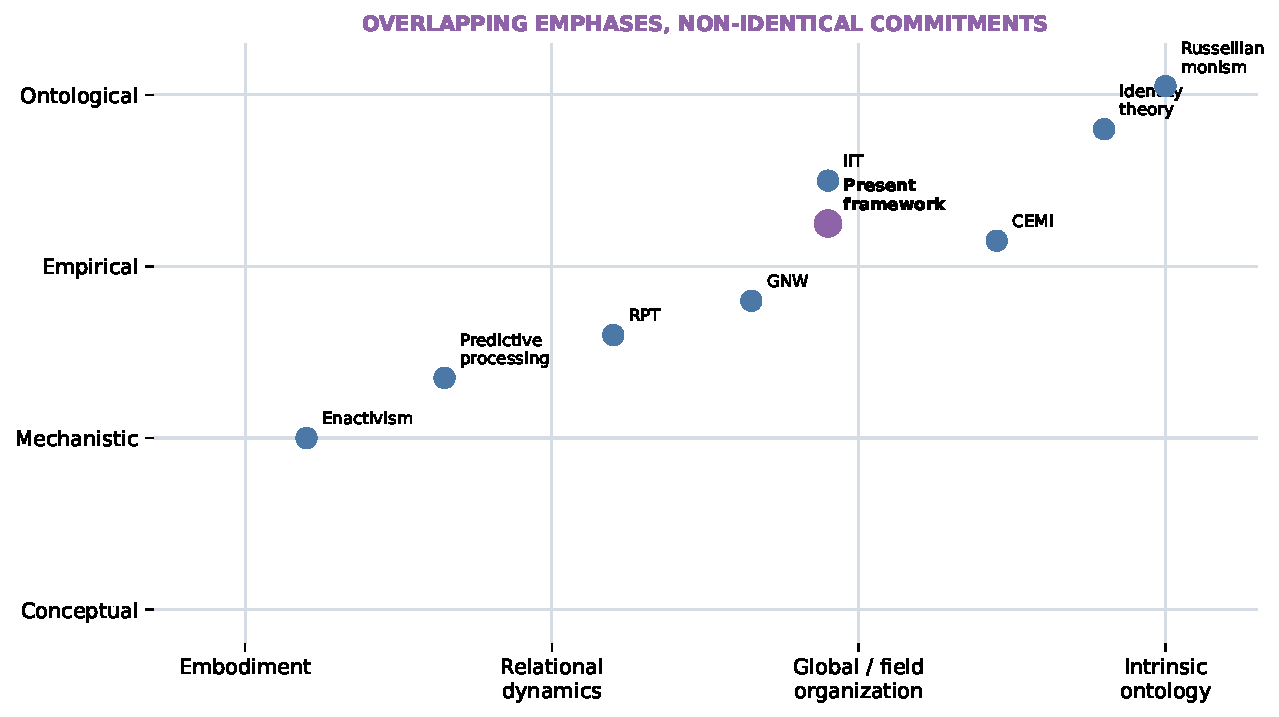
\includegraphics[width=0.88\linewidth,height=\textheight,keepaspectratio,alt={Neighbouring theories contribute at different levels. Overlap does not make their ontological commitments interchangeable.}]{figures/figure4_theory_matrix.pdf}
\caption{Neighbouring theories contribute at different levels. Overlap
does not make their ontological commitments interchangeable.}
\end{figure}

\section{Experimental programme}\label{experimental-programme}

The programme is organized as seven linked lines. Each line can advance
without accepting the ontology. Shared methodological requirements
include preregistration where feasible, held-out validation, subject-
and dataset-level replication, explicit measurement models, comparison
with strong baselines, sensitivity to estimator choice, and publication
of negative results.

\subsection{Programme A --- Stable percepts and
transitions}\label{programme-a-stable-percepts-and-transitions}

Bistable perception, binocular rivalry, backward masking, near-threshold
detection, temporal integration, and confidence judgements provide
repeated transitions between perceptual organizations under similar
stimulation. Simultaneous EEG/MEG, intracranial recordings where
available, eye tracking, and trial-level reports can estimate ACS
before, during, and after transitions. Models should compare multiscale
ACS features with firing rate or amplitude, spectral power, anatomy,
standard static and dynamic connectivity, stimulus properties, eye
movements, and behaviour.

The central test is prospective: can relational trajectories predict
when a percept stabilizes, how long it dwells, and when it changes on
held-out trials and participants? Analyses should separate report
preparation from perceptual organization through no-report or
delayed-report contrasts where defensible. Failure of ACS to add
reproducible predictive value would weaken the central empirical
hypothesis.

\subsection{Programme B --- Qualia-related relational
signatures}\label{programme-b-qualia-related-relational-signatures}

Parametric colour, pitch, timbre, tactile, pain, and body-state continua
can test whether reported similarity corresponds to structured ACS
transformations. Designs should collect nonverbal similarity judgements
as well as labels, repeat stimuli across contexts, and estimate
within-subject reliability before attempting cross-subject alignment.
Relational geometry can be compared with raw activation geometry using
representational-similarity methods \citep{nili2014}.

The output should be called a candidate organizational correlate or
physical signature. Cross-subject convergence would not establish
identical experience, and language-specific boundaries must not be
mistaken for neural discontinuities.

\subsection{Programme C --- Consciousness level and
profile}\label{programme-c-consciousness-level-and-profile}

Wakefulness, REM and non-REM sleep, graded sedation, anaesthesia,
seizures, coma and other disorders of consciousness, meditation, and
psychedelic states offer partially overlapping changes in
responsiveness, content, and temporal continuity. Dynamic coordination
has already differentiated some conscious and unresponsive states
\citep{demertzi2019, luppi2019}, while perturbational complexity can
remain informative when behaviour is absent
\citep{casali2013, sarasso2015}.

ACS analyses should not simply reproduce a binary label. They should
estimate a profile of persistence, differentiation, recurrence,
integration--segregation balance, and transition richness, then relate
it to independent indices, retrospective reports, behavioural
responsiveness, and clinical outcome. Training on one state contrast and
testing on other datasets is essential to avoid an anaesthetic- or
acquisition-specific marker.

\subsection{Programme D --- Lesions and reversible
perturbations}\label{programme-d-lesions-and-reversible-perturbations}

Focal damage, disconnection, stimulation, pharmacological manipulation,
and reversible inhibition can reveal causal dependencies obscured by
intact-system correlation. The target is not a one-region/one-quale map.
Studies should measure how perturbation changes multiscale organization,
dwell and transition structure, content, global level, recovery, and
compensation.

A causal ACS account predicts structured deformation: damage to a hub or
recurrent pathway should affect specific profile dimensions and recovery
routes. Longitudinal data can distinguish immediate loss, homeostatic
compensation, and learned reorganization. Interventions should be chosen
with clinical and ethical constraints foremost.

\subsection{Programme E --- Neural cultures and organoid
systems}\label{programme-e-neural-cultures-and-organoid-systems}

In vitro preparations allow progressive construction of coupling:
spontaneous culture; patterned input; closed-loop stimulation;
differentiated sensory-like input layers; embodied robotic coupling; and
adaptive homeostatic control. Cortical organoids can develop structured
oscillatory activity \citep{trujillo2019}, and cultured neurons have
been placed in closed-loop simulated environments \citep{kagan2022}.
These results motivate measurement of dynamics, not claims of
consciousness.

At each stage, ask whether the system develops robust metastability,
perturbation recovery, hierarchical invariants, action-dependent
stabilization, and multiscale ACS. Comparisons require cell-type,
maturation, density, stimulation, and open-loop controls. Ethical
oversight should increase with functional complexity and uncertainty.
Behaviour-like adaptation or oscillation is insufficient to attribute
experience.

\subsection{Programme F --- Minimal physical
organization}\label{programme-f-minimal-physical-organization}

Excitable chemical media, coupled oscillators, neuromorphic circuits,
recurrent analog networks, active matter, and biological collectives can
clarify which properties are ubiquitous and which are distinctive. The
purpose is contrastive explanation. If nearly every dynamical system has
a rich-looking ACS under a flexible enough estimator, the construct
lacks specificity.

Matched perturbations should compare closure, recovery, counterfactual
sensitivity, hierarchy, controllability, and dependence on
self-maintenance variables. Minimal systems can falsify proposed
qualification criteria without being prematurely labelled conscious.

\subsection{Programme G --- Artificial embodied
agents}\label{programme-g-artificial-embodied-agents}

Artificial agents permit controlled ablation. Matched architectures can
differ in closed-loop coupling, persistent recurrent state, homeostatic
variables, multi-timescale memory, hierarchical invariant learning, and
local/global regulation. Environments should vary observation delay,
controllability, nuisance transformations, bodily damage or resource
variables, and distribution shift.

Outcomes include object permanence, transfer, perturbation robustness,
adaptation, self-maintenance, representation geometry, and ACS-like
organization. Matched parameter count and compute are necessary
baselines. Behavioural performance alone is insufficient to infer
consciousness; the programme tests the mechanistic chain.

\begin{figure}
\centering
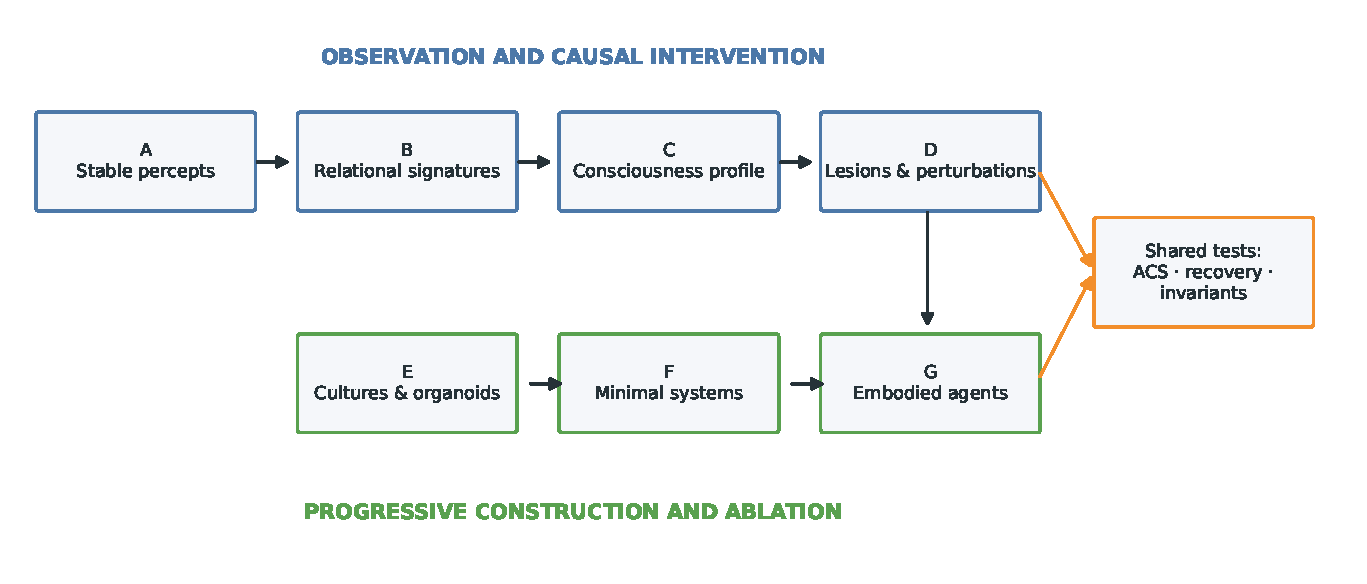
\includegraphics[width=0.95\linewidth,height=\textheight,keepaspectratio,alt={The experimental programmes move from human percepts and clinical states through perturbations to progressively constructed biological and artificial systems.}]{figures/figure5_experimental_programme.pdf}
\caption{The experimental programmes move from human percepts and
clinical states through perturbations to progressively constructed
biological and artificial systems.}
\end{figure}

\section{Operationalized predictions}\label{operationalized-predictions}

Each prediction specifies a paradigm, independent variable, dependent
measure, baseline, comparison, expected direction, disconfirmation
criterion, and theory specificity. Confirmation would primarily support
the mechanistic or empirical levels, not the identity thesis.

\subsection{P1 --- ACS adds predictive
value}\label{p1-acs-adds-predictive-value}

\begin{itemize}
\tightlist
\item
  \textbf{Dataset or paradigm:} preregistered near-threshold perception,
  masking, or binocular-rivalry EEG/MEG and intracranial datasets with
  trial-level reports.
\item
  \textbf{Independent variable:} perceived versus unperceived trials, or
  stable-percept versus transition periods, conditioned on stimulus and
  report demands.
\item
  \textbf{Dependent measure:} held-out AUC/log loss for report or
  transition prediction and explained variance in dwell time from
  multiscale ACS features.
\item
  \textbf{Baseline:} amplitude or firing rate, spectral power, anatomy,
  stimulus variables, eye movements, behaviour, and conventional
  single-window connectivity.
\item
  \textbf{Statistical comparison:} nested cross-validation with
  participant- and dataset-level random effects; likelihood-ratio or
  permutation tests for incremental value; correction for the tested ACS
  families.
\item
  \textbf{Expected direction:} ACS models improve out-of-sample
  prediction and calibration beyond all baselines.
\item
  \textbf{Disconfirmation:} no reproducible incremental value across at
  least two adequately powered datasets or gains vanish under
  leakage-free validation.
\item
  \textbf{Theory specificity:} supports the ACS empirical hypothesis
  more than generic theories that predict only activation or access; it
  does not distinguish all relational theories.
\end{itemize}

\subsection{P2 --- Cross-subject relational
convergence}\label{p2-cross-subject-relational-convergence}

\begin{itemize}
\tightlist
\item
  \textbf{Dataset or paradigm:} repeated naturalistic stimuli and
  controlled colour/object continua with functional or anatomical
  alignment.
\item
  \textbf{Independent variable:} matched versus mismatched perceptual
  organization across participants.
\item
  \textbf{Dependent measure:} cross-subject identification,
  representational-geometry correlation, or graph alignment in ACS space
  versus raw activation space.
\item
  \textbf{Baseline:} anatomical alignment, raw multivoxel or sensor
  activity, spectral features, stimulus-model embeddings, and label-only
  similarity.
\item
  \textbf{Statistical comparison:} held-out-subject decoding and
  permutation of stimulus identities; hierarchical bootstrap over
  participants and stimuli.
\item
  \textbf{Expected direction:} matched percepts align more strongly and
  generalize better in relational ACS space.
\item
  \textbf{Disconfirmation:} relational features fail to improve
  reliability or generalization, or improvements are fully explained by
  stimulus and label structure.
\item
  \textbf{Theory specificity:} tests the proposal that invariants are
  relationally organized; convergence remains a correlate rather than
  proof of shared qualia.
\end{itemize}

\subsection{P3 --- Hierarchical depth tracks invariant
cognition}\label{p3-hierarchical-depth-tracks-invariant-cognition}

\begin{itemize}
\tightlist
\item
  \textbf{Dataset or paradigm:} object, place, affordance, and concept
  tasks with controlled transformations and delayed sensorimotor
  contingencies.
\item
  \textbf{Independent variable:} transformation radius and temporal
  horizon required for generalization.
\item
  \textbf{Dependent measure:} timescale of ACS persistence, perturbation
  radius over which relational geometry is retained, and cross-condition
  decoding.
\item
  \textbf{Baseline:} model depth, receptive-field size, raw activity
  stability, direct supervised prediction accuracy, and static
  representational similarity.
\item
  \textbf{Statistical comparison:} mixed-effects trends across task
  demands and ablations; mediation of transfer by ACS persistence with
  prospective replication.
\item
  \textbf{Expected direction:} larger transformation radii and longer
  horizons recruit or learn structures stable across longer timescales
  and stronger perturbations.
\item
  \textbf{Disconfirmation:} invariant performance is consistently
  explained without increased multiscale persistence or perturbation
  tolerance.
\item
  \textbf{Theory specificity:} directly tests hierarchical invariant
  formation and the ``stable abstraction before prediction'' ordering.
\end{itemize}

\subsection{P4 --- Dynamic homeostasis supports sustained flexible
encoding}\label{p4-dynamic-homeostasis-supports-sustained-flexible-encoding}

\begin{itemize}
\tightlist
\item
  \textbf{Dataset or paradigm:} matched recurrent neural or
  embodied-agent models, with physiological validation where feasible,
  under prolonged input shifts and perturbations.
\item
  \textbf{Independent variable:} adaptive local/global regulation
  present, ablated, or replaced by fixed normalization.
\item
  \textbf{Dependent measure:} saturation and silence rates, effective
  dimensionality, entropy regime, task information, recovery time,
  transfer, and post-perturbation adaptability.
\item
  \textbf{Baseline:} equal-parameter models with no regulation, fixed
  gain, standard normalization, and regulation targeting only mean
  activity.
\item
  \textbf{Statistical comparison:} factorial ablation across seeds and
  environments with survival/time-to-failure analysis and held-out
  transfer tests.
\item
  \textbf{Expected direction:} regulated models spend more time in
  bounded informative regimes, recover faster, and generalize more
  robustly without collapsing variability.
\item
  \textbf{Disconfirmation:} regulation yields no robust benefit,
  equivalent baselines perform as well, or the predicted
  bounded-variability signature does not arise.
\item
  \textbf{Theory specificity:} tests dynamic rather than static
  homeostasis; benefits from any mechanism do not establish
  consciousness.
\end{itemize}

\subsection{P5 --- Consciousness level relates to a multidimensional ACS
profile}\label{p5-consciousness-level-relates-to-a-multidimensional-acs-profile}

\begin{itemize}
\tightlist
\item
  \textbf{Dataset or paradigm:} wakefulness, REM/NREM sleep, propofol
  and ketamine conditions, and independent disorders-of-consciousness
  cohorts.
\item
  \textbf{Independent variable:} state and independently assessed
  consciousness evidence, separated from behavioural responsiveness
  where possible.
\item
  \textbf{Dependent measure:} a preregistered ACS profile spanning
  persistence, differentiation, recurrence, integration--segregation
  dynamics, and transition richness.
\item
  \textbf{Baseline:} spectral power, static connectivity, anatomy, drug
  concentration, behavioural responsiveness, and PCI where available.
\item
  \textbf{Statistical comparison:} train on one or more state families
  and test on held-out families/sites; multivariate profile comparison
  rather than post hoc scalar construction.
\item
  \textbf{Expected direction:} independent consciousness evidence
  covaries with a reproducible configuration of dimensions, while
  different conscious states can occupy different regions of the
  profile.
\item
  \textbf{Disconfirmation:} the profile fails cross-state/site
  generalization or merely recovers responsiveness, drug, or acquisition
  differences.
\item
  \textbf{Theory specificity:} supports multiscale organization but may
  overlap with GNW, IIT, recurrent, and complexity-based theories;
  discriminating analyses must test their distinct measures.
\end{itemize}

\subsection{P6 --- Field effects are mediated by organized neural
dynamics}\label{p6-field-effects-are-mediated-by-organized-neural-dynamics}

\begin{itemize}
\tightlist
\item
  \textbf{Dataset or paradigm:} sham-controlled TMS, tACS, or other
  ethically accepted EM perturbation combined with high-density EEG/MEG
  and content/level measures.
\item
  \textbf{Independent variable:} perturbation waveform, location, phase,
  and intensity.
\item
  \textbf{Dependent measure:} content or confidence change; neural ACS
  change; field-model variables; direct, indirect, and residual effects.
\item
  \textbf{Baseline:} sham, active-control site/frequency, sensory
  side-effect ratings, source-level activity/power, and conventional
  connectivity.
\item
  \textbf{Statistical comparison:} preregistered multilevel
  causal-mediation models with measurement-error sensitivity and
  negative-control outcomes.
\item
  \textbf{Expected direction:} effects on content are mediated by
  measurable ACS changes; field variables add no stable residual
  prediction once sufficiently sensitive neural organization is
  included.
\item
  \textbf{Disconfirmation:} reproducible field-level residual effects
  survive measurement improvement, controls, and replication, or content
  changes systematically occur without detected ACS mediation.
\item
  \textbf{Theory specificity:} residual effects would favour independent
  causal-field theories over the manifestation view; full mediation
  would not establish that fields are irrelevant at all descriptive
  scales.
\end{itemize}

\subsection{P7 --- Embodied stabilization precedes broad task
optimization}\label{p7-embodied-stabilization-precedes-broad-task-optimization}

\begin{itemize}
\tightlist
\item
  \textbf{Dataset or paradigm:} delayed-control embodied agents trained
  across nuisance transformations and distribution shifts.
\item
  \textbf{Independent variable:} closed-loop self-stabilization with
  persistent state and viability variables versus matched feed-forward,
  open-loop, and reward-optimized controls.
\item
  \textbf{Dependent measure:} training time at which transferable
  invariant geometry, perturbation recovery, and object permanence
  emerge relative to peak benchmark performance.
\item
  \textbf{Baseline:} equal parameters, environment interactions,
  compute, augmentation, and optimized task reward.
\item
  \textbf{Statistical comparison:} time-resolved mixed-effects analysis
  across seeds/tasks and preregistered change-point ordering.
\item
  \textbf{Expected direction:} self-stabilizing agents acquire
  transferable invariant organization and robust recovery before maximal
  benchmark score, with a stronger ordering than controls.
\item
  \textbf{Disconfirmation:} no reproducible ordering or transfer
  advantage, or it disappears under matched optimization and data
  exposure.
\item
  \textbf{Theory specificity:} tests the developmental ordering implied
  by embodied stabilization; it bears no direct inference about
  artificial consciousness.
\end{itemize}

\section{Artificial intelligence and
PRAttention}\label{artificial-intelligence-and-prattention}

Current language models display complex learned representations and
internal dynamics. Most deployed systems, however, lack persistent
sensorimotor closure, organism-like viability regulation, and a
continuously self-maintained internal physical world. Behavioural
sophistication is therefore insufficient, under this framework, to infer
consciousness. The framework also does not prove that current AI is
unconscious: its qualification criteria are provisional, and
architecture-level evidence cannot settle an identity claim.

Future tests should examine persistent recurrent state, environmental
coupling, sensorimotor closure, self-maintenance variables, dynamic
homeostasis, multi-timescale memory, hierarchical invariant pickup,
endogenous goals constrained by viability, and perturbation-sensitive
ACS monitoring. These are design and measurement principles, not a
recipe guaranteed to produce experience.

Standard attention performs context-dependent binding among token
representations \citep{vaswani2017}. Retrieval-augmented systems add
selected external information \citep{lewis2020}. \textbf{PRAttention},
developed in companion engineering work, proposes explicit reference
handles and progressive retrieval into persistent referential
structures. This may extend effective context and approximate one
component of hierarchical world maintenance: an agent can preserve a
reference, expand it when needed, and revisit an externalized structure.
PRAttention by itself lacks the full embodied, homeostatic, recurrent
organization described here. It is an engineering bridge, not a theory
or implementation of consciousness.

\section{Objections, alternatives, and
limitations}\label{objections-alternatives-and-limitations}

\subsection{Redescription objection}\label{redescription-objection}

\textbf{Objection.} ``Stabilization'' and ``ACS'' merely rename control
and connectivity without adding mechanism. \textbf{Response.} The
framework is useful only if its ordering claims, perturbation profiles,
and incremental predictions outperform existing descriptions. P1, P3,
P4, and P7 are designed accordingly. \textbf{Open problem.} The
companion mechanistic paper must specify local learning and regulatory
rules rather than rely on verbal unification.

\subsection{Boundary and qualification
objection}\label{boundary-and-qualification-objection}

\textbf{Objection.} The features of a qualifying organization are chosen
to fit familiar conscious systems. \textbf{Response.} The paper presents
a multidimensional candidate profile and minimal-system contrasts, not a
definition by stipulation. \textbf{Open problem.} Necessary, sufficient,
or probabilistic qualification criteria remain unavailable; this is the
central philosophical weakness.

\subsection{Sufficiency versus
correlation}\label{sufficiency-versus-correlation}

\textbf{Objection.} Even perfect ACS prediction would show correlation,
not sufficiency or identity. \textbf{Response.} Agreed. Perturbations
can strengthen causal inference about mechanism, but the ontology
requires independent argument. \textbf{Open problem.} Establish whether
interventions on relational organization produce the predicted content
and level changes without circularly selecting features from reports.

\subsection{Observer-relative scale and variable
selection}\label{observer-relative-scale-and-variable-selection}

\textbf{Objection.} ACS depends on parcellation, window, estimator, and
the observer's description. \textbf{Response.} Robustness across
reasonable transformations, modalities, and scales is a required
criterion. Causal and predictive invariance can reduce arbitrariness.
\textbf{Open problem.} Define equivalence classes of ACS descriptions
and limits on admissible coarse-graining.

\subsection{Multiple realizability and biological
specificity}\label{multiple-realizability-and-biological-specificity}

\textbf{Objection.} Either the view wrongly excludes non-biological
realizations or makes biology irrelevant. \textbf{Response.} It remains
open whether non-biological systems can reproduce the relevant causal
organization. Biological material may contribute mechanisms not captured
by coarse computational equivalence. \textbf{Open problem.} Develop
matched biological, neuromorphic, and simulated comparisons without
presuming substrate neutrality.

\subsection{Dreaming and paralysis}\label{dreaming-and-paralysis}

\textbf{Objection.} Conscious episodes occur without overt
perception--action closure. \textbf{Response.} The core claim is
developmental and organizational, not that each episode requires action.
Recurrent architecture can maintain a temporarily decoupled world, as
dream reports and anaesthetic dissociations caution \citep{sarasso2015}.
\textbf{Open problem.} Specify how much ongoing bodily and environmental
closure is required across development and maintenance.

\subsection{Feed-forward
consciousness}\label{feed-forward-consciousness}

\textbf{Objection.} Brief conscious content might arise from largely
feed-forward sweeps. \textbf{Response.} ACS does not assume every
relevant relation is long-range, but the framework predicts that
qualifying content depends on recurrence or on a recurrently prepared
organization. \textbf{Open problem.} High-temporal-resolution masking
and no-report paradigms must discriminate early feed-forward sufficiency
from later recurrent and report-related effects.

\subsection{EM epiphenomenon}\label{em-epiphenomenon}

\textbf{Objection.} If EM organization is only manifestation, including
it adds nothing. \textbf{Response.} It provides a physically continuous
measurement bridge and a contrast with independent-field theories. A
manifestation can be empirically informative without being separately
sufficient. \textbf{Open problem.} P6 must address source uncertainty
and the possibility that field and generator descriptions cannot be
cleanly separated.

\subsection{Combination, decomposition, and subject
unity}\label{combination-decomposition-and-subject-unity}

\textbf{Objection.} Restricting experience to organized systems does not
explain why one ACS is one subject, how modules combine, or when
coupling merges subjects. \textbf{Response.} The objection is valid;
``solved by construction'' would overstate the case. Counterfactual
causal integration, shared homeostasis, and common perturbation recovery
are candidate boundary constraints. \textbf{Open problem.} A principled
individuation theory is required.

\subsection{Causal closure and scientific usefulness of
identity}\label{causal-closure-and-scientific-usefulness-of-identity}

\textbf{Objection.} An identity claim adds no causal prediction and is
scientifically idle. \textbf{Response.} Its direct role is conceptual:
it blocks a misleading production model and constrains which physical
organization is proposed as the referent of experience. Empirical
predictions arise from the mechanism, not metaphysical identity alone.
\textbf{Open problem.} Show that the identity framing guides non-trivial
boundary cases without merely redescribing results.

\subsection{Language-game continuity versus phenomenal
continuity}\label{language-game-continuity-versus-phenomenal-continuity}

\textbf{Objection.} Binary language can describe a genuinely
discontinuous phenomenon. \textbf{Response.} Agreed. The language-game
thesis explains conceptual pressure but supplies no evidence for
continuity. The continuity case must come from graded mechanisms and
structured transitions. \textbf{Open problem.} Determine whether ACS
profiles contain genuine discontinuities, hysteresis, or phase
transitions.

\subsection{AI behavioural imitation without
experience}\label{ai-behavioural-imitation-without-experience}

\textbf{Objection.} An artificial system could imitate every report
while lacking the proposed organization, or reproduce selected ACS
measures through engineering. \textbf{Response.} Report and behavioural
success are insufficient; implementation, closure, maintenance, and
perturbation response must also be examined. \textbf{Open problem.} No
behavioural or ACS test currently licenses certainty about artificial
experience, so ethical inference should remain explicitly uncertain.

\section{Research programme and companion
papers}\label{research-programme-and-companion-papers}

The foundation paper should remain independent of unfinished
simulations. Companion projects can develop: local learning,
self-perturbation, homeostasis, and hierarchy formation; comparison of
ACS estimators and graph/information measures; controlled embodied-agent
experiments; preregisterable neuroscience protocols and public-data
pipelines; PRAttention and persistent referential state; and
philosophical work on qualification, unity, intrinsic existence, and
identity.

Priority for v0.3 is not more scope. It is sharper formalism and
evidence: specify stabilization dynamics; define ACS equivalence and
scale selection; preregister P1 and P4 analyses; strengthen the
literature review; and clarify which observations discriminate this
framework from recurrent, workspace, integration, and field theories.

\section{Conclusion}\label{conclusion}

The framework proposes that cognition begins neither with passive input
nor with an isolated prediction objective, but with an embodied system
continually maintaining viable relations under perturbation. Dynamic
homeostasis preserves bounded activity and future adaptability. Repeated
stabilization across transformations produces hierarchical invariants
and an organism-centred internal physical world. Multiscale
activation-correlation structures provide a provisional relational
language for connecting neural events, metastable population
organization, behaviour, phenomenological transitions, and measurable
electromagnetic manifestations.

The empirical wager is demanding but ordinary: ACS profiles must add
reproducible, out-of-sample value beyond stronger and simpler baselines,
survive changes of estimator and dataset, and respond to perturbation as
predicted. Failure should narrow or reject the construct. The
ontological wager is more speculative: a qualifying organized physical
world does not generate an additional observer or substance; its
intrinsic existence is hypothesized to be the subjective aspect. This
relocates rather than solves the hard problem and leaves qualification
and unity unresolved.

The programme's value therefore does not depend on declaring the
metaphysics complete. It lies in keeping mechanism, evidence, and
ontology connected without collapsing them---and in making the
distinctive links precise enough to test, criticize, and revise.

\bibliography{references.bib}

\end{document}
